\documentclass{standalone}
\usepackage{tikz}
\usepackage{tikz-qtree}
\usepackage[makeroom]{cancel}
\usetikzlibrary{fit}


\begin{document} 
	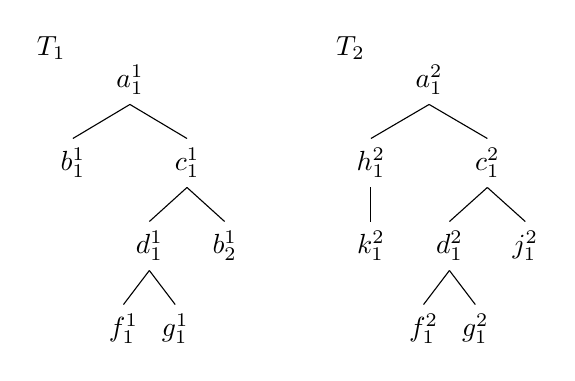
\begin{tikzpicture}[]

	    \node (x) at (-1,0.5) {$T_1$};
	    \Tree [.$a^1_1$
	            [.$b^1_1$ ] 
	            [.$c^1_1$ 
	                [.$d^1_1$ 
	                	[.$f^1_1$ ]
	                	[.$g^1_1$ ]
	                ]
	                [.$b^1_2$ ] 
	            ]
	          ]
	    

	    \begin{scope}[xshift=3.8cm]
		    \node (y) at (-1,0.5) {$T_2$} ;
		    \Tree [.$a^2_1$
		            [.$h^2_1$ 
		            	[.$k^2_1$ ]
		            ] 
		            [.$c^2_1$ 
		                [.$d^2_1$ 
		                	[.$f^2_1$ ]
		                	[.$g^2_1$ ]
		                ]
		                [.$j^2_1$ ] 
		            ]
		          ]
	    \end{scope}


	\end{tikzpicture}
\end{document} 